\documentclass{article}
\usepackage{listings, verbatim}
\usepackage[usenames,dvipsnames]{color}
\usepackage[usenames,dvipsnames,svgnames,table]{xcolor}
\usepackage{amsmath,amsfonts,graphicx,comment,typearea,amsthm}
\usepackage{xcomment,psfrag,enumerate,scrpage2,xspace,hyperref,rotating,float}
\begin{document}

\title{MAS8381: Marketing Data Project}
\author{Michael Dunne-Willows:\\
Antonia Kontaratou:\\
Hayley Moore: 110331287}
\maketitle

\section{Converting the Variables}
We started our analysis by deciding whether a variable should be converted into a factor. We decided that if the variable was categorical, only had a small number of values and was unordered then to convert the variable to a factor. Table~\ref{variables} shows the variables an whether they are used as a factor or not.
\begin{table}[H]
\centering
\begin{tabular}{|l|l|}
\hline
\textbf{Variable} &\textbf{Used as}\\
\hline
Income       &Continuous variable  \\
Sex          &Factor with 2 levels \\
Marital      &Factor with 5 levels \\
Age          &Continuous variable  \\
Edu          &Factor with 6 levels\\
Occupation   &Factor with 9 levels\\
Lived        &Factor with 5 levels\\
Dual\_Income &Factor with 3 levels\\
Household    &Continuous variable  \\
Householdu18 &Continuous variable  \\
Status       &Factor with 3 levels \\
Home\_Type   &Factor with 5 levels \\
Ethnic       &Factor with 8 levels \\
Language     &Factor with 3 levels \\
\hline
\end{tabular}
\caption{variables}
\label{variables}
\end{table}
\noindent We had to just our judgement to set \textsf{Edu} and \textsf{Lived} as a factor as they were both ordered categorical variables. We decided that they should be classed as factors since in the case of education the gaps between levels were not consistent.
\\\\
We also decided that \textsf{Household} and \textsf{Householdu18} should be used as continuous variables since the gaps between each level were consistent this time. For example looking at the \textsf{Householdu18} information below
\begin{verbatim}
Householdu18 : PERSONS IN HOUSEHOLD UNDER 18 
0. None 1. One 2. Two 3. Three 4. Four 5. Five 6. Six 7. Seven 
8. Eight 9. Nine or more
\end{verbatim}
we can see that each gap is equivalent to one more under 18 person living in the house.


\section{handling missing data}
\label{handling}
\section{Frequ}
\section{Bayesian}
\subsection{Saturated Model}
We start the Bayesian analysis by modelling the saturated model with the missing data handled by just simply omitting it, later on we use the mice method mentioned earlier to handle the missing values. We have chosen to use a vague prior on each of our parameters, $\beta_i$, and for the precision, $\tau$. The model string  for this is 
\begin{verbatim}
modelstring = "
model {
for (i in 1:n) {
mean[i] =  inprod(X[i,],beta)
y[i]~dnorm(mean[i],tau)
}
for (j in 1:p) {
beta[j]~dnorm(0,0.001)
}
tau~dgamma(1,0.001)
}
"
\end{verbatim}
The MCMC had a burn in of 1000 iterations and a run of 10,000 iterations. From the plots of $\beta_1$ to $\beta_4$ we can see that the distribution converged. This is shown in Figure~\ref{saturated_beta1-4} by the "furry caterpillar" effect we see.
\begin{figure}[H]
\centering
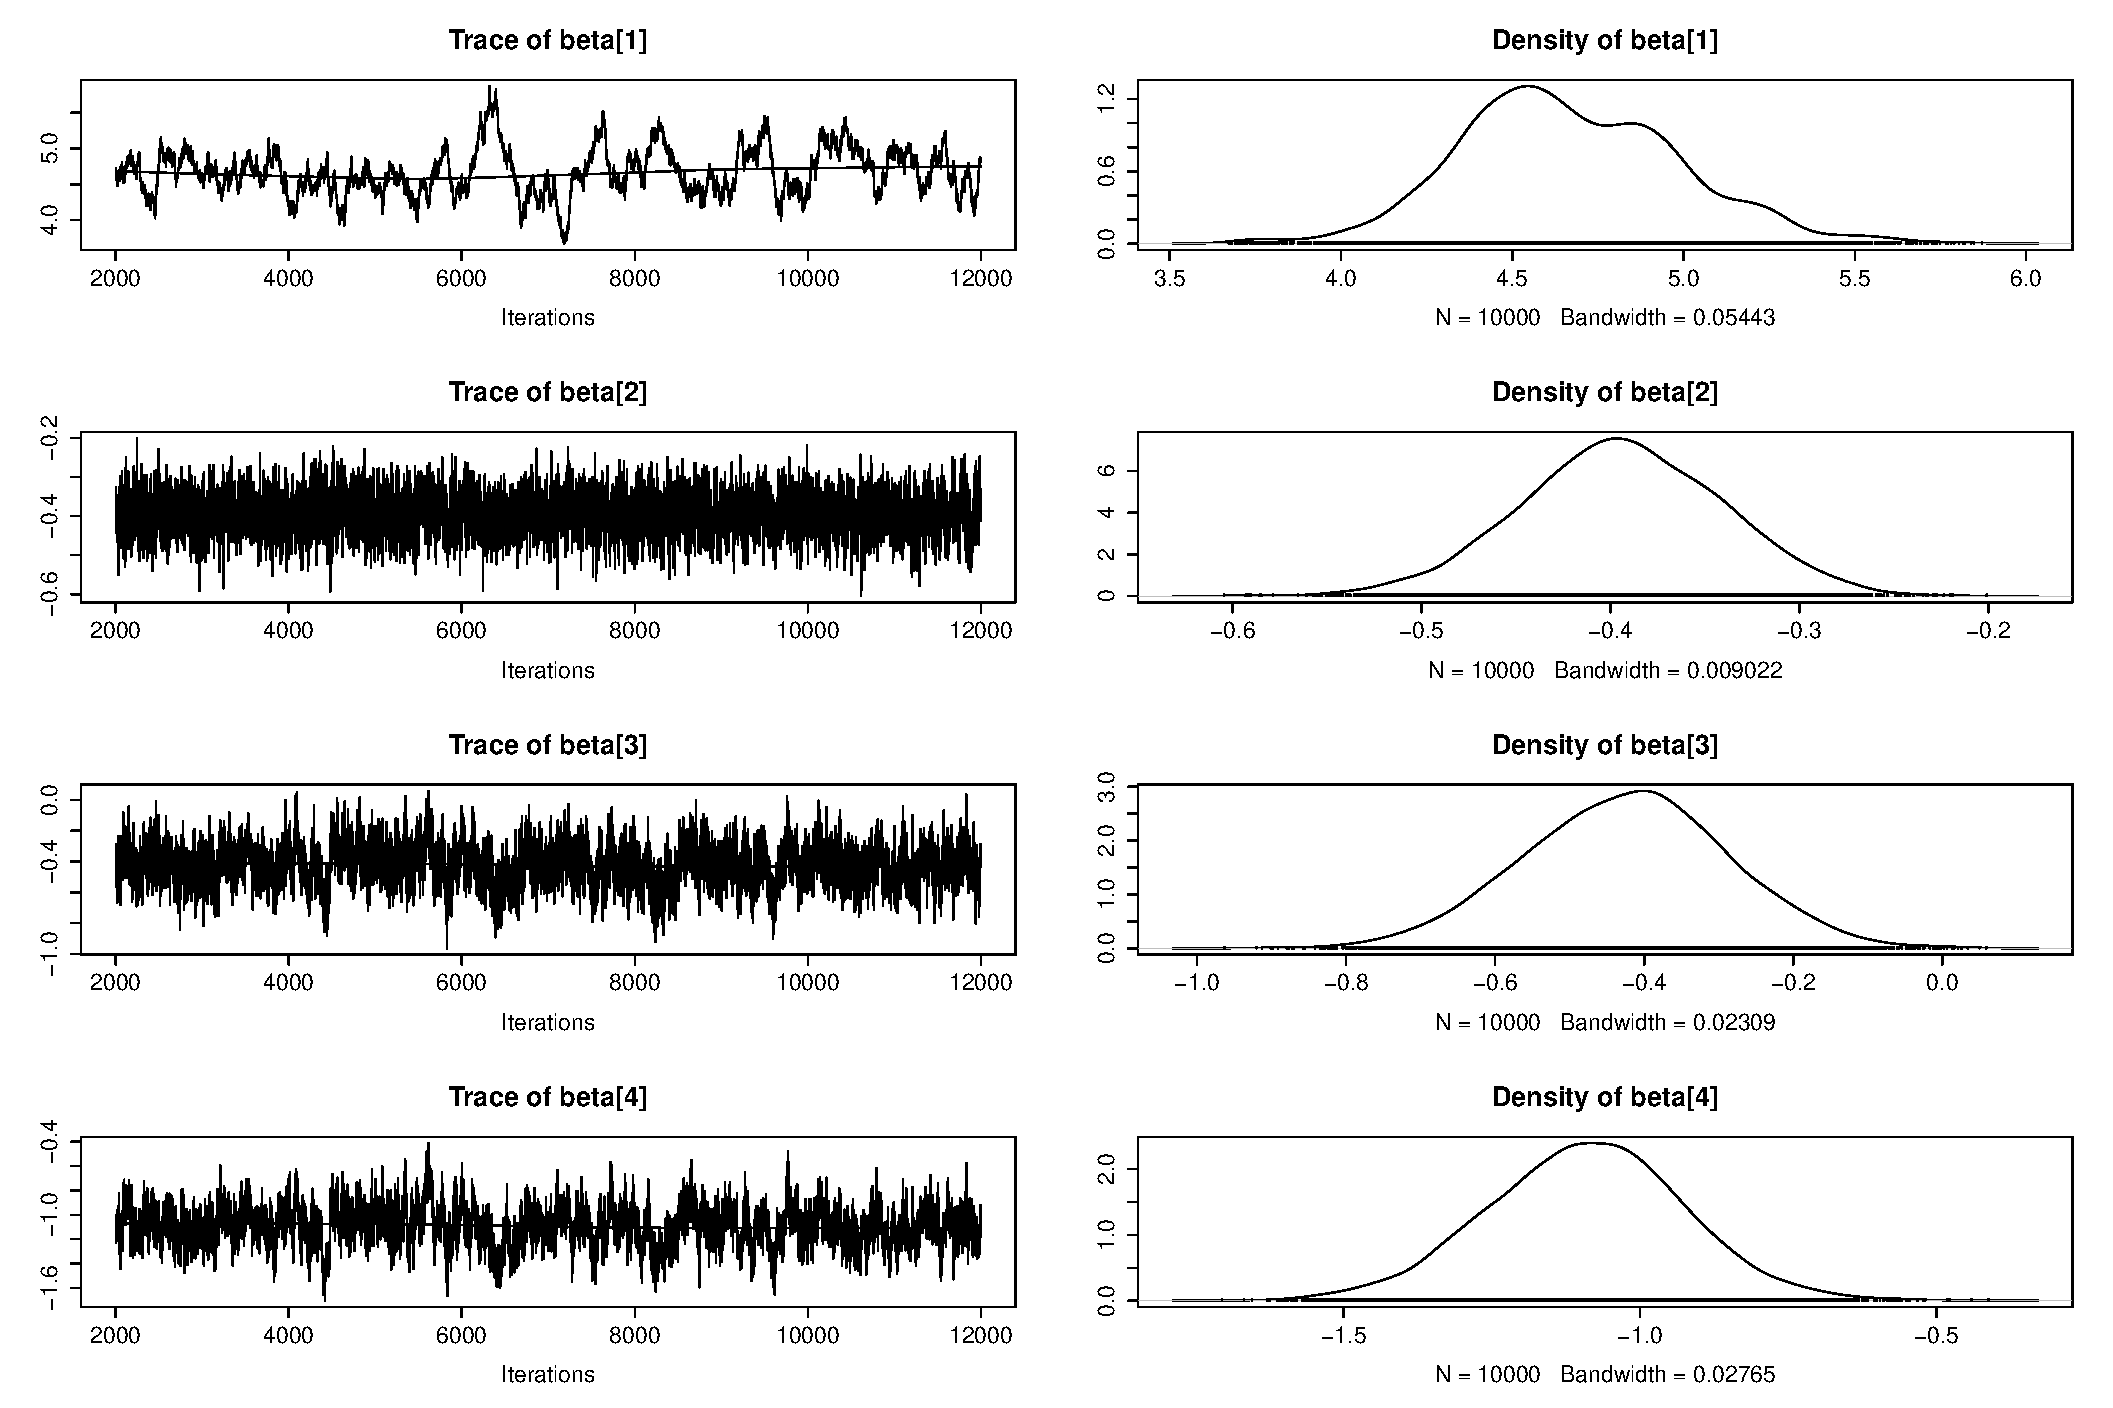
\includegraphics[width = 0.9\textwidth]{saturatedOutput/beta1-4.pdf}
\caption{Trace and density plots for the parameters $\beta_1, \beta_2, \beta_3$ and $\beta_4$.}
\label{saturated_beta1-4}
\end{figure}
\subsection{Variable Selection Model}
The model can be improved upon by using a model that does variable selection and random effects with prior inclusion. This means that the model will no longer have all the variables which will give us a model which is less likely to over fit and will have less bias. The random effects means that the variable value is now changed with a variable probability where the probability comes from a normal distribution. The model string we used to incorporate this is
\begin{verbatim}
modelstring = "
model{
for(i in 1:n){
mean[i] = inprod(X[i,], beta)
y[i] ~ dnorm(mean[i],tau)
}
for (j in 1:p) {
ind[j] ~ dbern(pind)
betaT[j] ~ dnorm(0,taub)
beta[j] = ind[j]*betaT[j]
}
tau ~ dgamma(1, 0.001)
taub ~ dgamma(1, 0.001)
pind ~ dbeta(2,8)
}
"
\end{verbatim}
we used this model to the data where the missing values had been replaced using the MICE method mention in Section~\ref{handling}


\end{document}